%%
%% This is file `sample-sigconf.tex',
%% generated with the docstrip utility.
%%
%% The original source files were:
%%
%% samples.dtx  (with options: `all,proceedings,bibtex,sigconf')
%% 
%% IMPORTANT NOTICE:
%% 
%% For the copyright see the source file.
%% 
%% Any modified versions of this file must be renamed
%% with new filenames distinct from sample-sigconf.tex.
%% 
%% For distribution of the original source see the terms
%% for copying and modification in the file samples.dtx.
%% 
%% This generated file may be distributed as long as the
%% original source files, as listed above, are part of the
%% same distribution. (The sources need not necessarily be
%% in the same archive or directory.)
%%
%%
%% Commands for TeXCount
%TC:macro \cite [option:text,text]
%TC:macro \citep [option:text,text]
%TC:macro \citet [option:text,text]
%TC:envir table 0 1
%TC:envir table* 0 1
%TC:envir tabular [ignore] word
%TC:envir displaymath 0 word
%TC:envir math 0 word
%TC:envir comment 0 0
%%
%% The first command in your LaTeX source must be the \documentclass
%% command.
%%
%% For submission and review of your manuscript please change the
%% command to \documentclass[manuscript, screen, review]{acmart}.
%%
%% When submitting camera ready or to TAPS, please change the command
%% to \documentclass[sigconf]{acmart} or whichever template is required
%% for your publication.
%%
%%
\documentclass[sigconf,authorversion,nonacm]{acmart}
%%
%% \BibTeX command to typeset BibTeX logo in the docs
\AtBeginDocument{%
  \providecommand\BibTeX{{%
    Bib\TeX}}}

%% Per SIGBOVIK request:
\usepackage{nopageno}

\usepackage{svg}
\usepackage{bytefield}
\usepackage{ulem}


%% Rights management information.  This information is sent to you
%% when you complete the rights form.  These commands have SAMPLE
%% values in them; it is your responsibility as an author to replace
%% the commands and values with those provided to you when you
%% complete the rights form.
% \setcopyright{acmlicensed}
% \copyrightyear{2018}
% \acmYear{2018}
% \acmDOI{XXXXXXX.XXXXXXX}
%% These commands are for a PROCEEDINGS abstract or paper.
\acmConference[SIGBOVIK '25]{ACH Special Interest Group on Harry Quire Bovik}{April 4, 2025}{Pittsburgh, PA}
%%
%%  Uncomment \acmBooktitle if the title of the proceedings is different
%%  from ``Proceedings of ...''!
%%
%%\acmBooktitle{Woodstock '18: ACM Symposium on Neural Gaze Detection,
%%  June 03--05, 2018, Woodstock, NY}
%\acmISBN{978-1-4503-XXXX-X/2018/06}


%%
%% Submission ID.
%% Use this when submitting an article to a sponsored event. You'll
%% receive a unique submission ID from the organizers
%% of the event, and this ID should be used as the parameter to this command.
%%\acmSubmissionID{123-A56-BU3}

%%
%% For managing citations, it is recommended to use bibliography
%% files in BibTeX format.
%%
%% You can then either use BibTeX with the ACM-Reference-Format style,
%% or BibLaTeX with the acmnumeric or acmauthoryear sytles, that include
%% support for advanced citation of software artefact from the
%% biblatex-software package, also separately available on CTAN.
%%
%% Look at the sample-*-biblatex.tex files for templates showcasing
%% the biblatex styles.
%%

%%
%% The majority of ACM publications use numbered citations and
%% references.  The command \citestyle{authoryear} switches to the
%% "author year" style.
%%
%% If you are preparing content for an event
%% sponsored by ACM SIGGRAPH, you must use the "author year" style of
%% citations and references.
%% Uncommenting
%% the next command will enable that style.
%%\citestyle{acmauthoryear}


%%
%% end of the preamble, start of the body of the document source.
\begin{document}

%%
%% The "title" command has an optional parameter,
%% allowing the author to define a "short title" to be used in page headers.
\title{HTTP offload is a \sout{dumb} great idea whose time has come}

%%
%% The "author" command and its associated commands are used to define
%% the authors and their affiliations.
%% Of note is the shared affiliation of the first two authors, and the
%% "authornote" and "authornotemark" commands
%% used to denote shared contribution to the research.
\author{Charles Eckman}
\authornote{This was Charles' idea.}
\author{Stephen Longfield}

%%
%% By default, the full list of authors will be used in the page
%% headers. Often, this list is too long, and will overlap
%% other information printed in the page headers. This command allows
%% the author to define a more concise list
%% of authors' names for this purpose.
\renewcommand{\shortauthors}{Eckman et al.}

%%
%% The abstract is a short summary of the work to be presented in the
%% article.
\begin{abstract}

%Application-specific hardware acceleration is becoming more in more common in hyperscaler datacenters.
%Many of these hyperscalers serve data on HTTP endpoints.
%And just like other dumb ideas whose time has come\cite{mogul2003tcp}, now it is HTTP's turn.

%In this paper, we implemented a \sout{fully} functional HTTP endpoint on FPGA, using the Amaranth HDL.
%This allows us to fully implement RFC2324 and RFC7168, creating a circuit with both special-purpose electrical components designed to heat tea and serve HTTP.

% TODO: Incorporate
% Implemented \st{fully} functional HTTP peripheral in Amaranth hardware, synthesized for FPGA
% Something about Coffee/Tea
% HTTP offload per se is neither of much overall benefit nor free from significant costs and risks. 

% Remixed from TCP offload paper

Since time immemorial, providers of hypertext services have dreamed of making their servers better.
One effective technique for accomplishing making software faster and stronger is to implement it \textit{harder},\cite{murphy2022harder}
that is, to offload processing from a CPU into a dedicated hardware device.
This technique has been used for lower layers of the network stack, but for hypertext,
they have been mere fantasies, met with unjustified disdain.
We show that HTTP offload is an effective technique for addressing truly vital, very specific goals,
including performance, efficiency, and preparation of hot beverages.

Just like other ideas whose time has come\cite{mogul2003tcp}, now it is HTTP's turn to be offloaded into hardware.

\end{abstract}

%%
%% The code below is generated by the tool at http://dl.acm.org/ccs.cfm.
%% Please copy and paste the code instead of the example below.
\begin{CCSXML}
<ccs2012>
   <concept>
       <concept_id>10002951.10003260.10003304.10003306</concept_id>
       <concept_desc>Information systems~RESTful web services</concept_desc>
       <concept_significance>500</concept_significance>
       </concept>
   <concept>
       <concept_id>10010583.10010600.10010628.10010629</concept_id>
       <concept_desc>Hardware~Hardware accelerators</concept_desc>
       <concept_significance>500</concept_significance>
       </concept>
 </ccs2012>
\end{CCSXML}

\ccsdesc[500]{Information systems~RESTful web services}
\ccsdesc[500]{Hardware~Hardware accelerators}


%%
%% Keywords. The author(s) should pick words that accurately describe
%% the work being presented. Separate the keywords with commas.
\keywords{FPGA, HTTP, Good Ideas}

%%
%% This command processes the author and affiliation and title
%% information and builds the first part of the formatted document.
\maketitle

\section{Introduction}

Originally, "computing" was something done in a person's head.
Over time, the computing industry has steadily offloaded computation
from general-purpose computers (e.g. brains) into specialized hardware artifacts
(e.g. Napier's bones, bomba kryptologiczna, Furby). In recent years,
specialized hardware has provided acceleration for bitcoin mining (SHA hashing),
machine learning (matrix-multiply units), and video encoding (hardware codecs).

Accelerating network protocols has proven a fruitful domain for acceleration-
focusing on a common horizontal, rather than a vertical. Today's high-end NICs
and routers have dedicated hardware for Ethernet PHY, IP forwarding,
TCP offloading, and even TLS offloading.

To our knowledge, however, network acceleration has stalled out at OSI layer 6.\footnote{Not that we looked very hard.}
While running HTTP on embedded devices is common \cite{esp-idf-http-server},
"offload" onto another processor does not provide the full benefits of hardware acceleration.
We set out to complete the walk up the OSI stack, and create an HTTP server in hardware.\footnote{
Due to time and budget constraints, "hardware" means an FPGA. Anyone want to sponsor us for Tiny Tapeout?\cite{tinytapeout}
}

\section{Background}

\subsection{Fomu}

The specific hardware we chose to use as the platform for our HTTP implementation was the 
Fomu\cite{fomu} platform, chosen as the authors already owned them.

This platform contains an iCE40UP5K FPGA, which is well supported by open source toolchains. 
It has RGB LEDs, which are essential for the blinking light needed on every proper peice of hardwares~\cite{jargonfile_blinkenlights}.
The serial-over-USB interface is supports isn't perfect for HTTP, but the authors make it work.

Apart from all of these conveniences, the Fomu has the added advantage of being short and stout, which will come in handy later.

% TODO:  -- Done
% Fomu drives serial-over-USB constraints
% Offers a wide variety of network and real-world access opportunities. RGB LED
% The fomu form-factor is short and stout, which will come in handy later.

\subsection{Amaranth}

The hardware definition was implemented using Amaranth HDL\cite{amaranth}, selected for its code readability and virtue of appearing far earlier in alphabetical listings than competitors Verilog and VHDL.

This language contains many useful primitives, such as ready-valid channels,
as well as a built-in simulator supporting unit testing of modules.

As the Amaranth language is built on top of Python, we were able to integrate with the 
Hypothesis\cite{MacIver2019Hypothesis} testing library to get property-based testing, and
py\_test\cite{pytest8.3} for unit testing.

\section{Engineering}

The Fomu device only has USB for input and output. As such, we did not implement all the network layers up to HTTP.
Here we describe the portion of the transport layer used to bridge the Internet to the Fomu, and handling of the HTTP in hardware.

\subsection{nTCP}

In our HDL design, we began with the LUNA USB stack \cite{luna} because it was the first USB stack we could get working.
We configured the Fomu to present itself as a USB serial device (USB CDC ACM FTW).

While HTTP/1 and HTTP/2 are designed to run over TCP, a TCP connection is not quite the same as a serial stream.
A TCP connection includes explicit setup and teardown messages, allowing each party to detect the start and end of stream;
HTTP/1.0 (\cite{rfc1945}) makes use of this to find the start and end of each request. Lacking these brackets, HTTP/1.1 is subject to request smuggling,\cite{request-smuggling} a security failure which precludes all serious websites from using HTTP/1.1.

% https://texdoc.org/serve/bytefield.pdf/0
\begin{figure}[h]
\begin{bytefield}[bitwidth=1.1em]{24}
\bitheader{0,8,9,10,16,24} \\
\bitbox{8}{Stream ID} & \bitbox{1}{S} & \bitbox{1}{E} & \bitbox{1}{D} & \bitbox{5}{reserved} & \bitbox{8}{Body length} \\
\wordbox[lrt]{1}{Body} \\ 
\skippedwords \\
\wordbox[lrb]{1}{}
\end{bytefield}
\caption{nTCP packet layout}
\label{fig:ntcp-header}
\end{figure}

\begin{table*}[htp]
\centering
\begin{tabular}{|p{0.45\textwidth}|p{0.45\textwidth}|}
\hline
\textbf{HTTP Request} & \textbf{HTTP Response} \\
\hline
\begin{verbatim}POST /led HTTP/1.0\r\n
Host: test\r\n
User-Agent: chartreuse.org\r\n
Content-Type: text/plain\r\n
\r\n
7FFF00\r\n\end{verbatim} & 
\begin{verbatim}HTTP/1.0 200 OK\r\n
Host: Fomu\r\n
Content-Type: text/plain; charset=utf-8\r\n
\r\n
Thank you!\r\n\end{verbatim} \\
\hline
\end{tabular}
\caption{HTTP/1.0 Request and Response Pair}
\label{fig:http-request-example}
\end{table*}

We therefore decided to adopt HTTP/1.0 semantics ("one request per connection"), and built a small protocol
called "Not TCP" on top of the serial line. As shown in Figure~\ref{fig:ntcp-header}, each Not TCP packet consists of a 3-byte header followed by a variable-length body. The header provides a stream ID, allowing multiplexing requests to the device; flags, indicating the start (\texttt{S}), end (\texttt{E}) and direction (\texttt{D}) of the request/response; and the length of the body following the header.


% |           |   111111 | 1  2        |
% | 0..7      | 89012345 | 6..3        | ...
% | stream ID | SEDxxxxx | body length | body

% S: Start bit; first packet in a new request/response
% E: End bit; last packet in this request/response
% D: Direction bit; 0 means packet is directed to the accelerator, 1 means packet is directed to the host.

A program running on the USB host provides higher-level networking connectivity (TCP acceptance)
and bridges the resulting request and response streams to the Fomu device over Not TCP.
Put more simply, the host program is a logic inverter: it turns TCP into Not TCP and vice versa.

\subsection{HTTP Parsing in Hardware}

% TODO:
% Could rephrase/cut down. Somewhat repetative from the above
% Or heading: "another advantage of nTCP having one request per connection"

%% OLD
% For the purposes of SIGBOVIK (tomfoolery), the authors limited their parsing to HTTP/1.0. 
% Without persistent connections, each request-response transaction is a separate nTCP connection, so no state 
% needs to persist between transactions in the HTTP module.

Without the persistent connections of later revisions, HTTP/1.0 can be implemented in a pure dataflow manner, with no need to maintain state between nTCP transactions. This allowed the authors to simplify their implementation to fit in the LUT constraints of the Fomu, and the time constraints of publication.

Additionally, in HTTP/1.0, headers are just strongly encouraged, with none being strictly required.
We take advantage of that by completely ignoring headers in requests, and only producing
them in responses when we feel like it.

Figure~\ref{fig:http-request-parsing} shows the dataflow diagram, where double-lines
are used to show ready-valid channels that carry individual characters.

\begin{figure}[htbp]
\includesvg[width=0.45\textwidth]{images/http_parse_sigbovik.drawio.svg}
\caption{HTTP Request Parsing Workflow Diagram}
\label{fig:http-request-parsing}
\end{figure}

One of our endpoints allows users to \texttt{POST} a hex color to the Fomu's LEDs.
An example request/response might look like Table~\ref{fig:http-request-example}, which would 
set the LEDs to a brilliant shade of green.\footnote{In practice, the Fomu's red channel is much stronger than the green channel, resulting in a sweeter, softer, lower-ABV yellow.}

In this example, the start line parser would validate the start line, and pull out the \texttt{POST} method and \texttt{/led} path.
The headers would be summarily discarded, and the remainder of the message would be forwarded to the LED body parser to pull out the colors and decide on a response.
Once the response has been sent to the output channel, the nTCP session would end and the HTTP module would be ready for another request.

More complex responses (e.g., the \texttt{/count} endpoint, which responds with internal diagnostic counts) require
more data to flow from the body parser to the responders. Drawing those lines in Figure~\ref{fig:http-request-parsing}
is left as an exercise for the reader. Crayons may be provided upon request.

\subsection{RFC2324 and RFC7168}

% TODO:
% Jokes in here could be tightened up.

The IETF defined the Hyper Text Coffee Pot Control Protocol, HTCPCP/1.0 in RFC2324\cite{rfc2324},
and expanded on it in RFC7168\cite{rfc7168}.
These documents define how an HTTP server should respond if it is a teapot.

This naturally leads to the question: What, exactly, \textit{is} a teapot?

RFC2324 indicates that a teapot MAY have a \texttt{body} that is short and stout.
RFC7168 further indicates that TEA capable pots are "expected to heat water through the use of electric elements".

Merriam-Webster defines a teapot as a vessel in which tea is brewed and served~\cite{mw:teapot}.
Previous implementers have put software HTCPCP servers for code 418 in a teapot~\cite{error418net}, or have 
glued a commercial teapot on top of a laptop running an HTTP server~\cite{joereddington418}.
These implementers follow RFC2324's recommendation of being short and stout, but they do not follow RFC7168's expectation
to heat water through the use of an electric element.
While hyperscalers have shown through their use of evaporative cooling that HTTP-serving hardware can be used to evaporate water
(hence the term of art, cloud computing), this excessive degree of heating is counter to the purpose of the Hyper 
Text Coffee Pot Control Protocol (not to mention the Kyoto one).


\begin{figure*}[htb]
    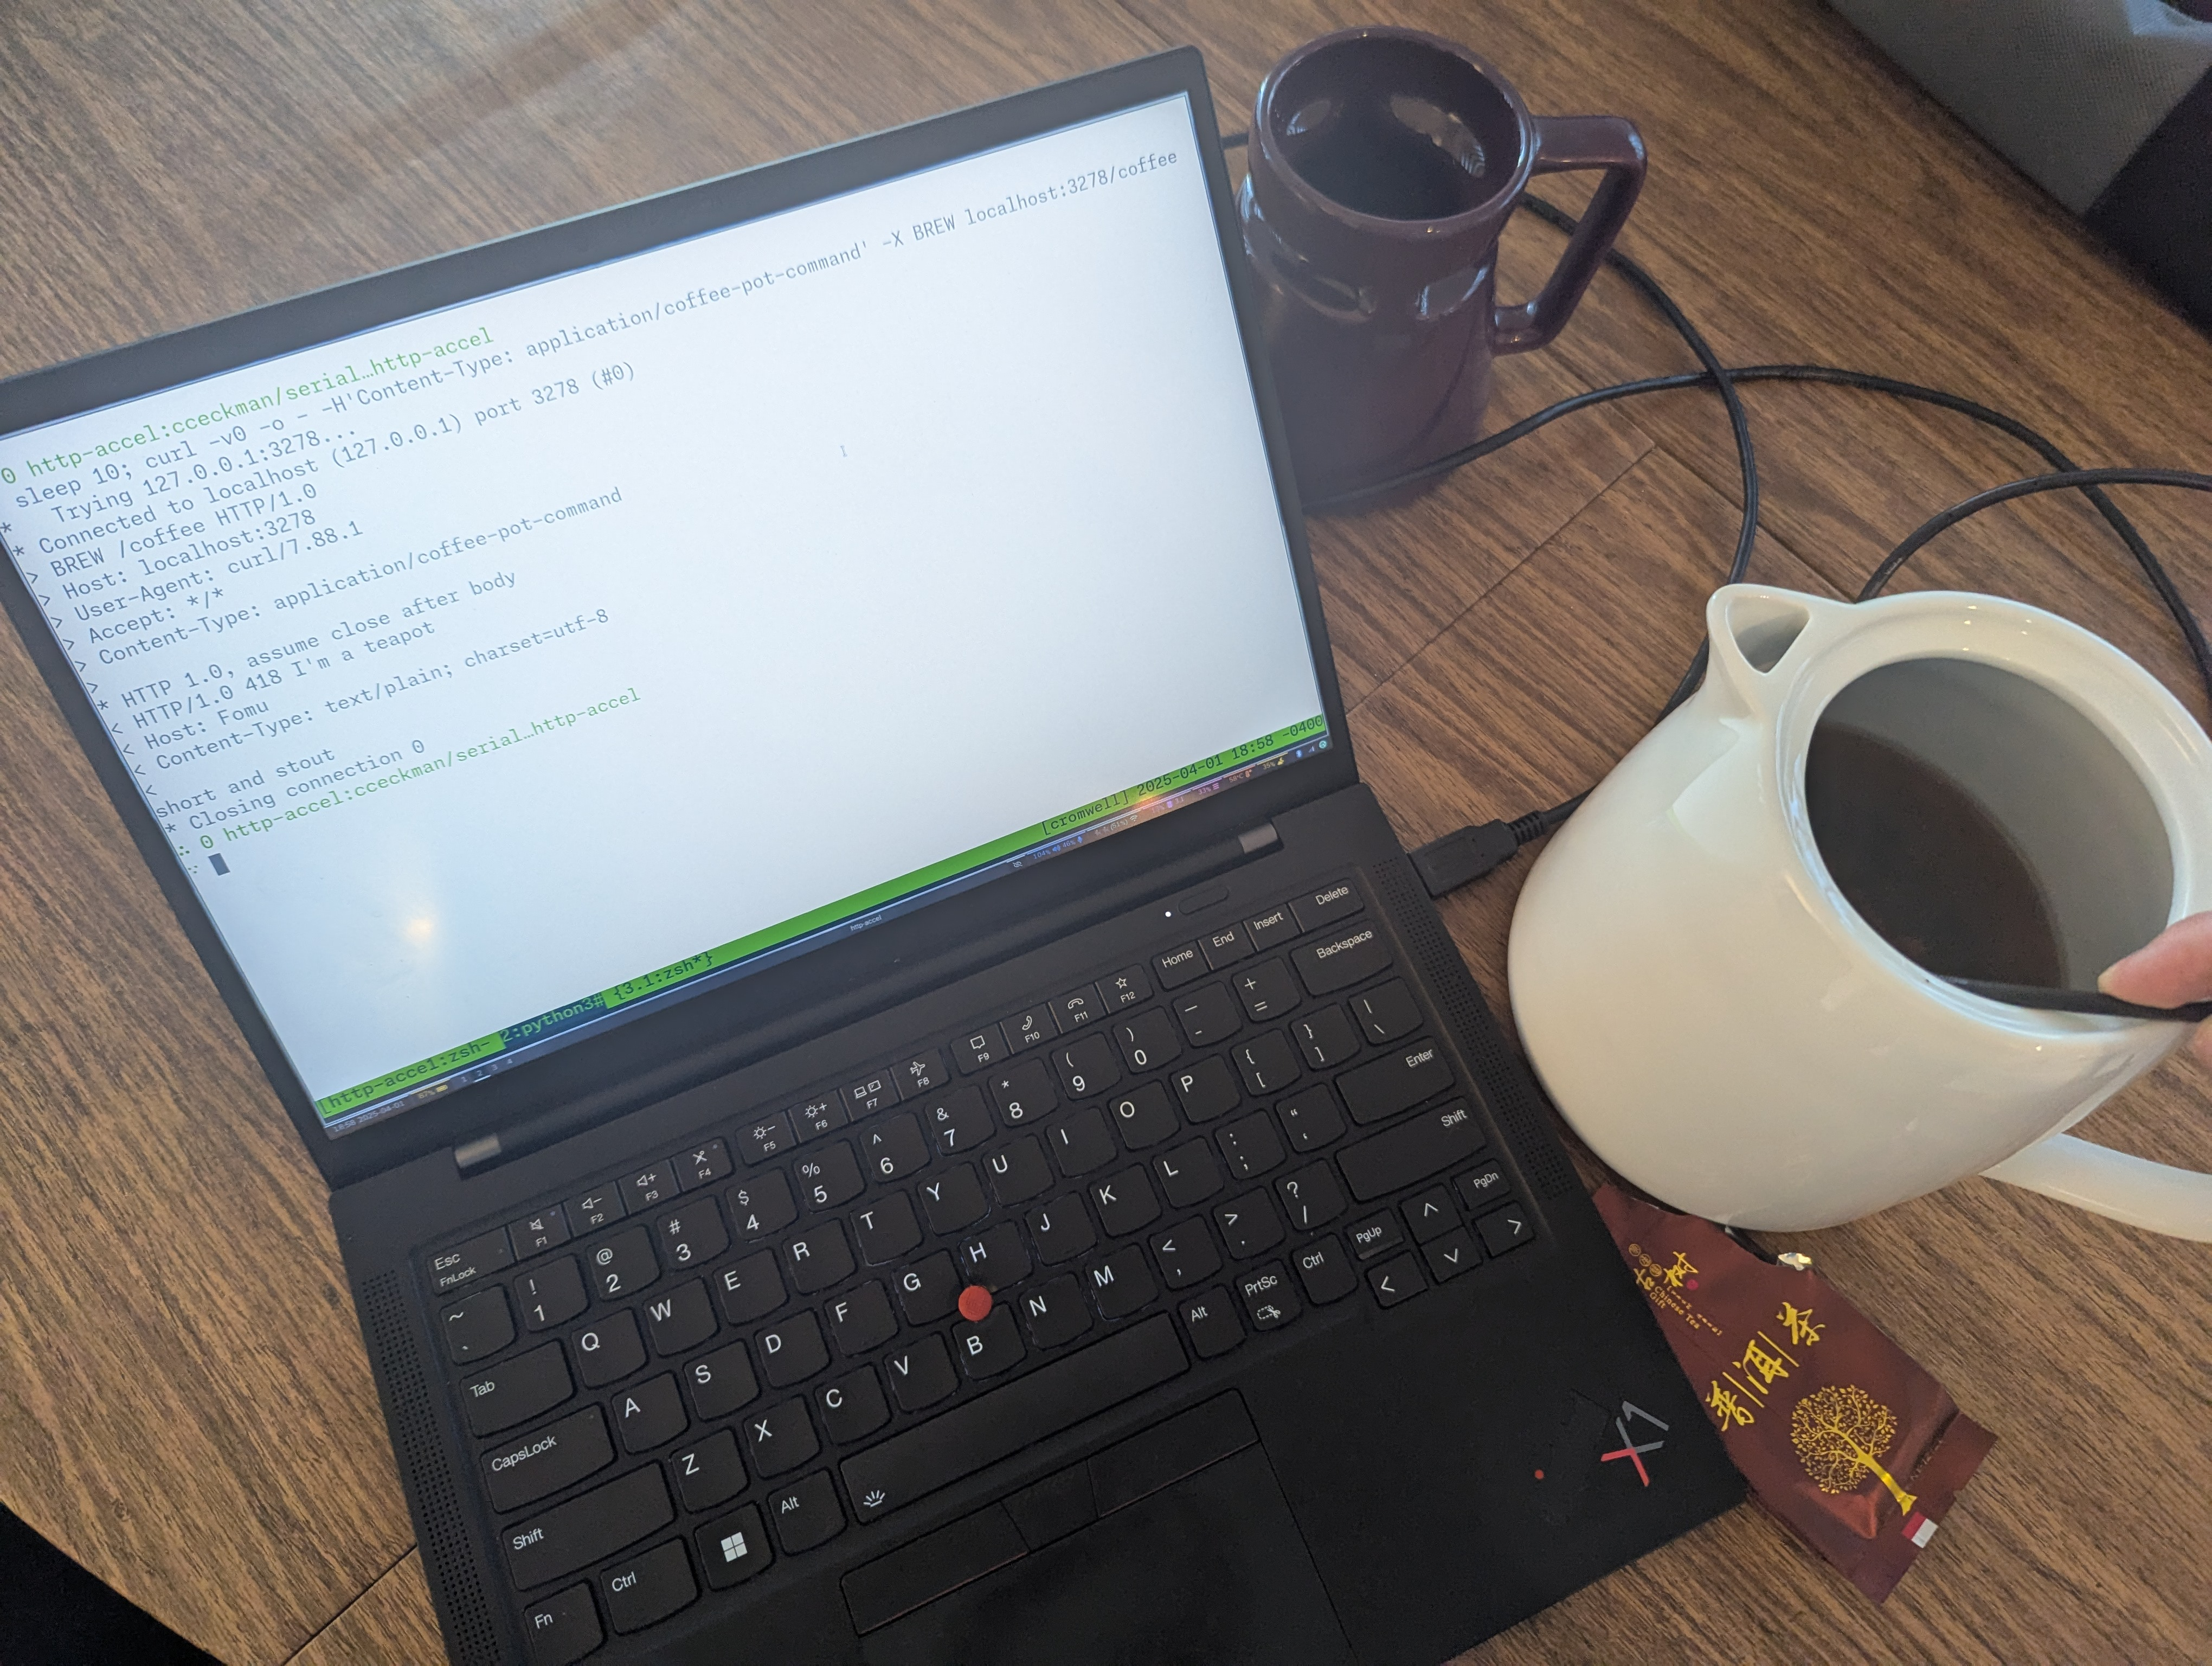
\includegraphics[width=0.8\textwidth]{images/htcpcp.jpg}
    \caption{RFC2324 compatibility tested (and tasted)}
    \label{fig:htcpcp}
\end{figure*}

As a more power-efficient and decentralized alternative, the authors added support for the \texttt{/coffee} path,
and serve \texttt{HTTP 418 I'm a teapot} responses.
The heat generated from serving these requests can be used to warm tea (note: energy transfer was minimal, but non-zero).
Therefore, the authors have created special-purpose electronics that serve the dual purpose of responding to 
RFC2324 requests while heating tea, making this the first RFC7168-compliant HTTP 418 endpoint we're aware of.


% TODO(cceckman): Hold some tea up to the FOMU, get a 418 response so the previous sentence is true.

\section{Results}

% TODO: How much of the Fomu did we end up using? What kind of performance did we see?

The resulting design uses a nice fraction of logic cells (3684 of the Fomu's 5280) and a small number of RAMs (5 of 30). Timing closes at 48MHz (USB logic) and 12MHz (main logic) with overhead to spare (51MHz and 21MHz, respectively).

% Info: Device utilisation:
% Info:            ICESTORM_LC:    3684/   5280    69%
% Info:           ICESTORM_RAM:       5/     30    16%
% Info:                  SB_IO:       7/     96     7%
% Info:                  SB_GB:       8/      8   100%
% Info:           ICESTORM_PLL:       0/      1     0%
% Info:            SB_WARMBOOT:       0/      1     0%
% Info:           ICESTORM_DSP:       2/      8    25%
% Info:         ICESTORM_HFOSC:       1/      1   100%
% Info:         ICESTORM_LFOSC:       0/      1     0%
% Info:                 SB_I2C:       0/      2     0%
% Info:                 SB_SPI:       0/      2     0%
% Info:                 IO_I3C:       0/      2     0%
% Info:            SB_LEDDA_IP:       0/      1     0%
% Info:            SB_RGBA_DRV:       0/      1     0%
% Info:         ICESTORM_SPRAM:       0/      4     0%


\section{Future work}

See TODOs at \url{https://github.com/cceckman/http-accel}. In accordance with RFC 9759\cite{rfc9759}, we expect all outstanding work in this area to be completed within two weeks.

\section{Conclusions}

% TODO: Add stuff about impact.

In conclusion, we managed to put an HTTP server on a Fomu FPGA platform using nTCP and other ETLAs.

Considering the industry's trend towards specialized hardware and AIASS (Artificial Intelligence AS a Service), developers of application accelerators should consider integrating the product's IP, TCP, HTTP, JSON parsing, APIs, storage, bot protection, authentication, A/B testing, billing, safety, and legal obligations into the hardware design.

%%
%% The acknowledgments section is defined using the "acks" environment
%% (and NOT an unnumbered section). This ensures the proper
%% identification of the section in the article metadata, and the
%% consistent spelling of the heading.
\begin{acks}
Thanks to Q for supporting Charles while working on this.
Thanks to M+T for leaving Stephen enough sleep to work on this.
Thanks to Scout, Bin, Wolfgang, Ludwig, and Arya for their emotional support.
And last, but not least, thank you Harry Q. Bovik for giving us a venue for this nonsense.
\end{acks}

%%
%% The next two lines define the bibliography style to be used, and
%% the bibliography file.
\bibliographystyle{ACM-Reference-Format}
\bibliography{citations}

\end{document}
\endinput
%%
%% End of file `sample-sigconf.tex'.
